\documentclass[12pt,a4paper]{article}
\usepackage[utf8]{vietnam}
\usepackage{amsmath,amssymb}
\usepackage[a4paper,left=2cm,right=1.8cm,top=1.8cm,bottom=1.8cm]{geometry}
\usepackage{tikz}
\usepackage{array,tabularx,longtable}
\usepackage{enumitem}
\setlength{\parindent}{0pt}
\setlength{\parskip}{3pt}
\linespread{1.15}
\pagestyle{plain}

% Phương án trắc nghiệm: 4 phương án trên 1 dòng / 2 dòng / mỗi phương án 1 dòng
\newcommand{\bonpa}[4]{\par\noindent\begin{tabularx}{\linewidth}{@{\hspace{0.6cm}}XXXX@{}}
\textbf{A.} #1 & \textbf{B.} #2 & \textbf{C.} #3 & \textbf{D.} #4\end{tabularx}\par}
\newcommand{\haipa}[4]{\par\noindent\begin{tabularx}{\linewidth}{@{\hspace{0.6cm}}XX@{}}
\textbf{A.} #1 & \textbf{B.} #2\\ \textbf{C.} #3 & \textbf{D.} #4\end{tabularx}\par}
\newcommand{\motpa}[4]{\par\hspace*{0.6cm}\textbf{A.} #1\par\hspace*{0.6cm}\textbf{B.} #2\par
\hspace*{0.6cm}\textbf{C.} #3\par\hspace*{0.6cm}\textbf{D.} #4\par}
\newcommand{\cau}[1]{\par\medskip\textbf{Câu #1.}~}
\newcommand{\bai}[2]{\par\medskip\textbf{Bài #1} \textit{(#2)}.~}
\newcommand{\y}[1]{\par\hspace*{0.6cm}#1}
\newcommand{\phan}[1]{\par\bigskip{\large\textbf{#1}}\par\smallskip}
\setlength{\extrarowheight}{2pt}

\begin{document}
% ===================== ĐỀ SỐ 5 =====================
\noindent
\begin{minipage}[t]{0.38\linewidth}\centering
TRƯỜNG THCS \dotfill\\[2pt]
\textbf{ĐỀ SỐ 5}
\end{minipage}\hfill
\begin{minipage}[t]{0.6\linewidth}\centering
\textbf{ĐỀ KIỂM TRA GIỮA HỌC KÌ I}\\
\textbf{NĂM HỌC 2026 -- 2027}\\
\textbf{MÔN: TOÁN 7} -- Sách \textit{Kết nối tri thức với cuộc sống}\\
\textit{Thời gian làm bài: 90 phút (không kể thời gian giao đề)}
\end{minipage}

\medskip
Họ và tên: \dotfill\ Lớp: \makebox[2cm]{\dotfill}\ Số báo danh: \makebox[2.5cm]{\dotfill}
\phan{A. TRẮC NGHIỆM (3,0 điểm)}
\textbf{Phần I. Câu trắc nghiệm nhiều phương án lựa chọn} \textit{(1,0 điểm)}. Thí sinh trả lời từ câu 1 đến câu 4. Mỗi câu hỏi thí sinh chỉ chọn một phương án.
\cau{1} Số hữu tỉ lớn nhất trong các số sau là
\bonpa{$-0{,}6$}{$\dfrac{3}{10}$}{$-\dfrac{1}{2}$}{$\dfrac{2}{5}$}
\cau{2} Kết quả của phép tính $(-0{,}5)^{2}$ là
\bonpa{$0{,}25$}{$-0{,}25$}{$1$}{$-1$}
\cau{3} Phân số $\dfrac{5}{11}$ được viết dưới dạng số thập phân là
\bonpa{$0{,}45$}{$0{,}(45)$}{$0{,}4(5)$}{$0{,}(4)$}
\cau{4} Phần giả thiết của định lí “Nếu một đường thẳng cắt hai đường thẳng song song thì hai góc đồng vị bằng nhau” là
\motpa{Hai góc đồng vị bằng nhau.}{Hai đường thẳng song song.}{Một đường thẳng cắt hai đường thẳng song song.}{Một đường thẳng cắt hai đường thẳng.}

\medskip\textbf{Phần II. Câu trắc nghiệm đúng sai} \textit{(1,0 điểm)}. Trong mỗi ý a), b), c), d) ở câu 5, thí sinh chọn đúng hoặc sai.
\cau{5} Xét tính đúng, sai của các khẳng định sau:
\y{a) $\dfrac{7}{8}=0{,}875$.}
\y{b) Làm tròn số $12{,}467$ đến hàng phần mười ta được $12{,}4$.}
\y{c) $\dfrac{2}{3}=0{,}(6)$.}
\y{d) Phân số $\dfrac{3}{14}$ viết được dưới dạng số thập phân hữu hạn.}

\medskip\textbf{Phần III. Câu trắc nghiệm trả lời ngắn} \textit{(1,0 điểm)}. Thí sinh trả lời từ câu 6 đến câu 9.
\cau{6} Tính giá trị của biểu thức $\left(\dfrac{3}{2}\right)^{2}-\dfrac{1}{4}$.
\cau{7} Tìm $x$, biết $\dfrac{3}{5}-x=\dfrac{1}{10}$ (viết kết quả dưới dạng số thập phân).
\cau{8} Cho tam giác $ABC$ có $\widehat{A}=100^\circ$ và $\widehat{B}=\widehat{C}$. Tính số đo $\widehat{B}$ (đơn vị: độ).
\cau{9} Đường thẳng $c$ cắt hai đường thẳng song song $a$ và $b$. Biết hai góc trong cùng phía tạo thành có hiệu bằng $40^\circ$. Tính số đo góc lớn hơn (đơn vị: độ).
\phan{B. TỰ LUẬN (7,0 điểm)}
\bai{1}{1,0 điểm} Tính (hợp lí nếu có thể):
\par\noindent\begin{tabularx}{\linewidth}{@{\hspace{0.6cm}}XX@{}}a) $\dfrac{13}{17}\cdot\dfrac{-2}{5}+\dfrac{4}{17}\cdot\dfrac{-2}{5}-\dfrac{3}{5}$; & b) $\dfrac{2^{10}\cdot 3^{5}}{4^{4}\cdot 3^{4}}$.\end{tabularx}
\bai{2}{1,5 điểm} Tìm $x$, biết:
\y{a) $\dfrac{3}{4}+x=-\dfrac{1}{2}$;}
\y{b) $\left(\dfrac{2}{3}-x\right)\cdot\dfrac{5}{2}=\dfrac{5}{6}$;}
\y{c) $\left(x-\dfrac{1}{2}\right)\cdot\left(x+\dfrac{2}{3}\right)=0$.}
\bai{3}{1,0 điểm} Một bể nước dạng hình hộp chữ nhật có chiều dài $2{,}5$ m, chiều rộng $1{,}6$ m và chiều cao $1{,}2$ m. Lượng nước hiện có trong bể chiếm $\dfrac{3}{4}$ thể tích của bể. Hỏi cần bơm thêm bao nhiêu lít nước nữa để bể đầy? (Biết $1\,\mathrm{m}^{3}=1\,000$ lít.)
\bai{4}{1,5 điểm} Cho hình vẽ bên, đường thẳng $c$ cắt hai đường thẳng $a$, $b$ lần lượt tại $A$, $B$ và $\widehat{A_1}=\widehat{B_1}=110^\circ$.
\begin{center}
\begin{tikzpicture}[scale=1.15,line cap=round,line join=round]
  \draw[line width=0.7pt] (-0.300,2.000) -- (5.000,2.000);
  \draw[line width=0.7pt] (-0.300,0.000) -- (5.000,0.000);
  \draw[line width=0.7pt] (1.726,2.752) -- (3.002,-0.752);
  \node[anchor=west,inner sep=1pt] at (5.150,2.000) {$a$};
  \node[anchor=west,inner sep=1pt] at (5.150,0.000) {$b$};
  \node[anchor=west,inner sep=1pt] at (1.576,2.752) {$c$};
  \fill (2.000,2.000) circle (1.3pt);
  \node[anchor=center,inner sep=1pt] at (1.700,1.780) {$A$};
  \fill (2.728,0.000) circle (1.3pt);
  \node[anchor=center,inner sep=1pt] at (3.028,-0.220) {$B$};
  \draw[line width=0.5pt] (2.300,2.000) arc[start angle=0,end angle=110,radius=0.300];
  \node[anchor=center,inner sep=1pt] at (2.287,2.410) {{\small 1}};
  \draw[line width=0.5pt] (2.103,1.718) arc[start angle=-70,end angle=0,radius=0.300];
  \node[anchor=center,inner sep=1pt] at (2.410,1.713) {{\small 2}};
  \draw[line width=0.5pt] (3.028,0.000) arc[start angle=0,end angle=110,radius=0.300];
  \node[anchor=center,inner sep=1pt] at (3.015,0.410) {{\small 1}};
  \draw[line width=0.5pt] (2.625,0.282) arc[start angle=110,end angle=180,radius=0.300];
  \node[anchor=center,inner sep=1pt] at (2.318,0.287) {{\small 2}};
\end{tikzpicture}
\end{center}
\y{a) Chứng minh $a\parallel b$.}
\y{b) Tính số đo $\widehat{A_2}$ và $\widehat{B_2}$.}
\y{c) Tia phân giác của $\widehat{B_2}$ cắt đường thẳng $a$ tại $K$. Tính số đo $\widehat{AKB}$.}
\bai{5}{1,5 điểm} Cho hai tam giác $ABC$ và $DCB$ có $AB=DC$, $AC=DB$; hai điểm $A$ và $D$ nằm cùng phía đối với đường thẳng $BC$. Gọi $O$ là giao điểm của $AC$ và $BD$.
\y{a) Chứng minh $\triangle ABC=\triangle DCB$.}
\y{b) Chứng minh $\widehat{ABD}=\widehat{DCA}$.}
\y{c) Biết $\widehat{ACB}=40^\circ$. Tính số đo $\widehat{BOC}$ và $\widehat{AOB}$.}
\bai{6}{0,5 điểm} Tìm các số nguyên $x$ để biểu thức $A=\dfrac{2x+5}{x+1}$ có giá trị là số nguyên.

\bigskip\begin{center}\textbf{--------- HẾT ---------}\\
\textit{Giáo viên coi kiểm tra không giải thích gì thêm.}\end{center}

\newpage
\begin{center}{\large\textbf{HƯỚNG DẪN CHẤM -- ĐỀ SỐ 5}}\end{center}
\phan{A. TRẮC NGHIỆM (3,0 điểm)}
\textbf{Phần I.} Mỗi câu trả lời đúng được 0,25 điểm.

\begin{tabular}{|l|*{4}{>{\centering\arraybackslash}p{2cm}|}}\hline
Câu & 1 & 2 & 3 & 4 \\ \hline
Đáp án & \textbf{D} & \textbf{A} & \textbf{B} & \textbf{C} \\ \hline
\end{tabular}

\textbf{Phần II.} Mỗi ý trả lời đúng được 0,25 điểm.

\begin{tabular}{|l|*{4}{>{\centering\arraybackslash}p{2cm}|}}\hline
Câu 5 & a) & b) & c) & d) \\ \hline
Đáp án & \textbf{Đúng} & \textbf{Sai} & \textbf{Đúng} & \textbf{Sai} \\ \hline
\end{tabular}

\textbf{Phần III.} Mỗi câu trả lời đúng được 0,25 điểm.

\begin{tabular}{|l|*{4}{>{\centering\arraybackslash}p{2cm}|}}\hline
Câu & 6 & 7 & 8 & 9 \\ \hline
Đáp án & \textbf{2} & \textbf{0,5} & \textbf{40} & \textbf{110} \\ \hline
\end{tabular}

\phan{B. TỰ LUẬN (7,0 điểm)}
\begin{longtable}{|>{\bfseries}c|p{0.76\linewidth}|>{\centering\arraybackslash}p{1.3cm}|}\hline
Bài & \multicolumn{1}{c|}{\textbf{Nội dung}} & \textbf{Điểm} \\ \hline\endhead
1a & \rule{0pt}{4ex}$=\dfrac{-2}{5}\cdot\left(\dfrac{13}{17}+\dfrac{4}{17}\right)-\dfrac{3}{5}=\dfrac{-2}{5}\cdot 1-\dfrac{3}{5}$\rule[-2.4ex]{0pt}{0pt} & 0,25 \\ \hline
 & \rule{0pt}{4ex}$=-\dfrac{5}{5}=-1$\rule[-2.4ex]{0pt}{0pt} & 0,25 \\ \hline
1b & \rule{0pt}{4ex}$=\dfrac{2^{10}\cdot 3^{5}}{\left(2^{2}\right)^{4}\cdot 3^{4}}=\dfrac{2^{10}\cdot 3^{5}}{2^{8}\cdot 3^{4}}$\rule[-2.4ex]{0pt}{0pt} & 0,25 \\ \hline
 & $=2^{2}\cdot 3=12$ & 0,25 \\ \hline
2a & \rule{0pt}{4ex}$x=-\dfrac{1}{2}-\dfrac{3}{4}=-\dfrac{2}{4}-\dfrac{3}{4}$\rule[-2.4ex]{0pt}{0pt} & 0,25 \\ \hline
 & \rule{0pt}{4ex}$x=-\dfrac{5}{4}$. Vậy $x=-\dfrac{5}{4}$.\rule[-2.4ex]{0pt}{0pt} & 0,25 \\ \hline
2b & \rule{0pt}{4ex}$\dfrac{2}{3}-x=\dfrac{5}{6}:\dfrac{5}{2}=\dfrac{1}{3}$\rule[-2.4ex]{0pt}{0pt} & 0,25 \\ \hline
 & \rule{0pt}{4ex}$x=\dfrac{2}{3}-\dfrac{1}{3}=\dfrac{1}{3}$. Vậy $x=\dfrac{1}{3}$.\rule[-2.4ex]{0pt}{0pt} & 0,25 \\ \hline
2c & \rule{0pt}{4ex}$x-\dfrac{1}{2}=0$ hoặc $x+\dfrac{2}{3}=0$\rule[-2.4ex]{0pt}{0pt} & 0,25 \\ \hline
 & \rule{0pt}{4ex}$x=\dfrac{1}{2}$ hoặc $x=-\dfrac{2}{3}$. Vậy $x\in\left\{\dfrac{1}{2};-\dfrac{2}{3}\right\}$.\rule[-2.4ex]{0pt}{0pt} & 0,25 \\ \hline
3 & Thể tích của bể: $2{,}5\cdot 1{,}6\cdot 1{,}2=4{,}8$ ($\mathrm{m}^{3}$). & 0,25 \\ \hline
 & \rule{0pt}{4ex}Lượng nước hiện có trong bể: $4{,}8\cdot\dfrac{3}{4}=3{,}6$ ($\mathrm{m}^{3}$).\rule[-2.4ex]{0pt}{0pt} & 0,25 \\ \hline
 & Lượng nước cần bơm thêm: $4{,}8-3{,}6=1{,}2$ ($\mathrm{m}^{3}$). & 0,25 \\ \hline
 & Đổi $1{,}2\,\mathrm{m}^{3}=1\,200$ lít. Vậy cần bơm thêm $1\,200$ lít nước. & 0,25 \\ \hline
4a & Ta có $\widehat{A_1}=\widehat{B_1}=110^\circ$ & 0,25 \\ \hline
 & mà $\widehat{A_1}$ và $\widehat{B_1}$ ở vị trí đồng vị nên $a\parallel b$. & 0,25 \\ \hline
4b & $\widehat{A_2}=180^\circ-\widehat{A_1}=180^\circ-110^\circ=70^\circ$ (hai góc kề bù). & 0,25 \\ \hline
 & $\widehat{B_2}=180^\circ-\widehat{B_1}=180^\circ-110^\circ=70^\circ$ (hai góc kề bù). & 0,25 \\ \hline
4c & \rule{0pt}{4ex}Lấy điểm $E$ trên đường thẳng $b$ sao cho tia $BE$ là một cạnh của $\widehat{B_2}$. Vì $BK$ là tia phân giác của $\widehat{B_2}$ nên $\widehat{KBE}=\dfrac{70^\circ}{2}=35^\circ$.\rule[-2.4ex]{0pt}{0pt} & 0,25 \\ \hline
 & Vì $a\parallel b$ nên $\widehat{AKB}=\widehat{KBE}=35^\circ$ (hai góc so le trong). & 0,25 \\ \hline
5 & Vẽ hình, ghi GT – KL đúng. \newline \textit{(Hình vẽ ở cuối hướng dẫn chấm)} & 0,25 \\ \hline
5a & Xét $\triangle ABC$ và $\triangle DCB$ có: $AB=DC$ (gt); $AC=DB$ (gt); $BC$ là cạnh chung. & 0,25 \\ \hline
 & Do đó $\triangle ABC=\triangle DCB$ (c.c.c). & 0,25 \\ \hline
5b & Từ câu a: $\widehat{ABC}=\widehat{DCB}$ và $\widehat{ACB}=\widehat{DBC}$ (các góc tương ứng). Suy ra $\widehat{ABC}-\widehat{DBC}=\widehat{DCB}-\widehat{ACB}$, tức là $\widehat{ABD}=\widehat{DCA}$. & 0,25 \\ \hline
5c & $\widehat{OBC}=\widehat{DBC}=\widehat{ACB}=40^\circ$, $\widehat{OCB}=40^\circ$. Trong $\triangle OBC$: $\widehat{BOC}=180^\circ-40^\circ-40^\circ=100^\circ$. & 0,25 \\ \hline
 & $\widehat{AOB}=180^\circ-\widehat{BOC}=80^\circ$ (hai góc kề bù). & 0,25 \\ \hline
6 & \rule{0pt}{4ex}Điều kiện $x\neq -1$. Ta có $A=\dfrac{2(x+1)+3}{x+1}=2+\dfrac{3}{x+1}$. $A$ nguyên khi $3$ chia hết cho $x+1$.\rule[-2.4ex]{0pt}{0pt} & 0,25 \\ \hline
 & $x+1\in\{1;-1;3;-3\}$, suy ra $x\in\{0;-2;2;-4\}$ (thoả mãn). & 0,25 \\ \hline
\end{longtable}
\textit{Lưu ý: Học sinh làm cách khác đúng vẫn cho điểm tối đa theo thang điểm tương ứng. Bài hình không vẽ hình hoặc vẽ hình sai không chấm phần tương ứng.}

\textbf{Hình vẽ bài 5:}
\begin{center}
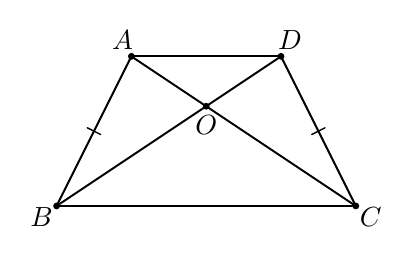
\begin{tikzpicture}[scale=0.95,line cap=round,line join=round]
  \draw[line width=0.7pt] (1.000,2.000) -- (0.000,0.000);
  \draw[line width=0.7pt] (0.000,0.000) -- (4.000,0.000);
  \draw[line width=0.7pt] (4.000,0.000) -- (3.000,2.000);
  \draw[line width=0.7pt] (1.000,2.000) -- (4.000,0.000);
  \draw[line width=0.7pt] (0.000,0.000) -- (3.000,2.000);
  \draw[line width=0.7pt] (1.000,2.000) -- (3.000,2.000);
  \draw[line width=0.5pt] (0.411,1.045) -- (0.589,0.955);
  \draw[line width=0.5pt] (3.411,0.955) -- (3.589,1.045);
  \fill (1.000,2.000) circle (1.3pt);
  \node[anchor=center,inner sep=1pt] at (0.880,2.220) {$A$};
  \fill (3.000,2.000) circle (1.3pt);
  \node[anchor=center,inner sep=1pt] at (3.120,2.220) {$D$};
  \fill (0.000,0.000) circle (1.3pt);
  \node[anchor=center,inner sep=1pt] at (-0.200,-0.150) {$B$};
  \fill (4.000,0.000) circle (1.3pt);
  \node[anchor=center,inner sep=1pt] at (4.200,-0.150) {$C$};
  \fill (2.000,1.333) circle (1.3pt);
  \node[anchor=center,inner sep=1pt] at (2.000,1.083) {$O$};
\end{tikzpicture}
\end{center}

\end{document}
